\scanpage{18}
8) Let now $\mathcal E^*$ be a graded ring, \deleted{equipped with} such that there exists $L\in\mathcal E^{(2)}$ satisfying the \uline{Lefschetz conditions} (\deleted{of} the conditions of the corollary of the preceding number\textsuperscript{o}). We say that $\mathcal E^*$ is a ``\deleted{Lefschetzian operator,}\inserted{Lefschetzian correspondence} ring'' (\unsure{this|this one} \deleted{\illegible{3}} \deleted{\unsure{with the system}} \unsure{at the number\textsuperscript{o}|of number\textsuperscript{o}} (even) as a Lefschetz system), and $L$ one of its ``Lefschetz elements''.
\deleted{\unsure{Outside} $(\unsure{\varphi(\Phi)=\mathcal E^*})$}
The associated element $\Lambda$ is \deleted{\unsure{called|called}} ``the \deleted{\unsure{adjoint for}} \deleted{\unsure{anti}}\inserted{co.}Lefschetzian element'' associated with $L$.
(NB. Note that $L$ is deduced from $\Lambda$ as $\Lambda$ from $L$, by simple symmetry on the degrees of $\mathcal E^*$ \deleted{$\unsure{\xi_0}$} $-$, and passage to the opposite ring --- \deleted{\unsure{transposed}} transposition isomorphism ---).
\margin{\figure{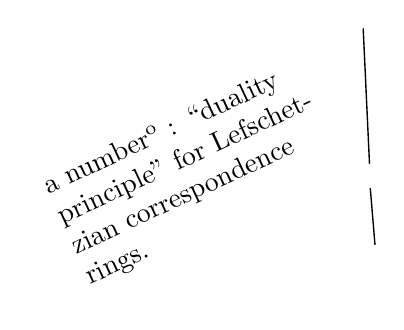
\begin{tikzpicture}
\node[align=left,text width=3.8cm,rotate=25] at (0,0) {a number\textsuperscript{o} : ``duality principle'' for Lefschetzian correspondence rings.};
\draw[line width=.5pt] (2.05,1.8)--(2.13,.08);
\draw[line width=.5pt] (2.14,-.23)--(2.2,-.95);
\end{tikzpicture}}}

One may ask to \uline{characterize} the \deleted{the} Lefschetz elements $L$. A necessary condition, when the number $2n$ is not redundant, i.e.
\[
\begin{aligned}
1)\quad&\mathcal E^{(2n)}\neq0\quad\deleted{\unsure{\{}}\quad(\Longrightarrow)\quad1')\ \mathcal E^{(-2n)}\neq0\quad\deleted{\unsure{\}}}\\
&(\Longrightarrow)\quad2)\ \pi_0,\deleted{\unsure{\pi_{2n}}}\neq0\quad\deleted{\unsure{\}}}
\end{aligned}
\]
\margin{\figure{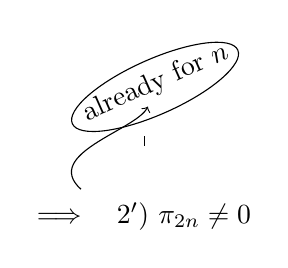
\begin{tikzpicture}
\node[align=left] at (0,0) {$\Longrightarrow\quad2')\ \pi_{2n}\neq0$};
\node[rotate=24] at (.15,1.7) {already for $n$};
\draw[rotate=24] (.8,1.45) ellipse (1.15cm and .35cm);
\draw[->] (-.8,.35) .. controls (-1.3,.8) and (-.1,1.1) .. (.05,1.4);
\draw (.01,1.02)--(.01,.9);
\end{tikzpicture}}}
that
\[
(\Longrightarrow)\quad3)\ L^n\neq0\quad(\Longrightarrow)\quad3')\ \Lambda^{\unsure{n|-}}\neq0\quad\deleted{\Longleftrightarrow}
\]
it is that one has $L^n\neq0$. One sometimes has a converse, in the case where ($\mathcal E$ being an \uline{algebra} over a commutative ring $k$)
\mspage{17}
